\documentclass[main]{subfiles}

\begin{document}

\section{Лекция 8}

Интуция гомотопической эквивалентности: например, круг без круга эквивалентен окружности, так как можно
<<схлопнуть>> кольцо вдоль радиусов и получить окружность.

\begin{figure}[H]
	\centering 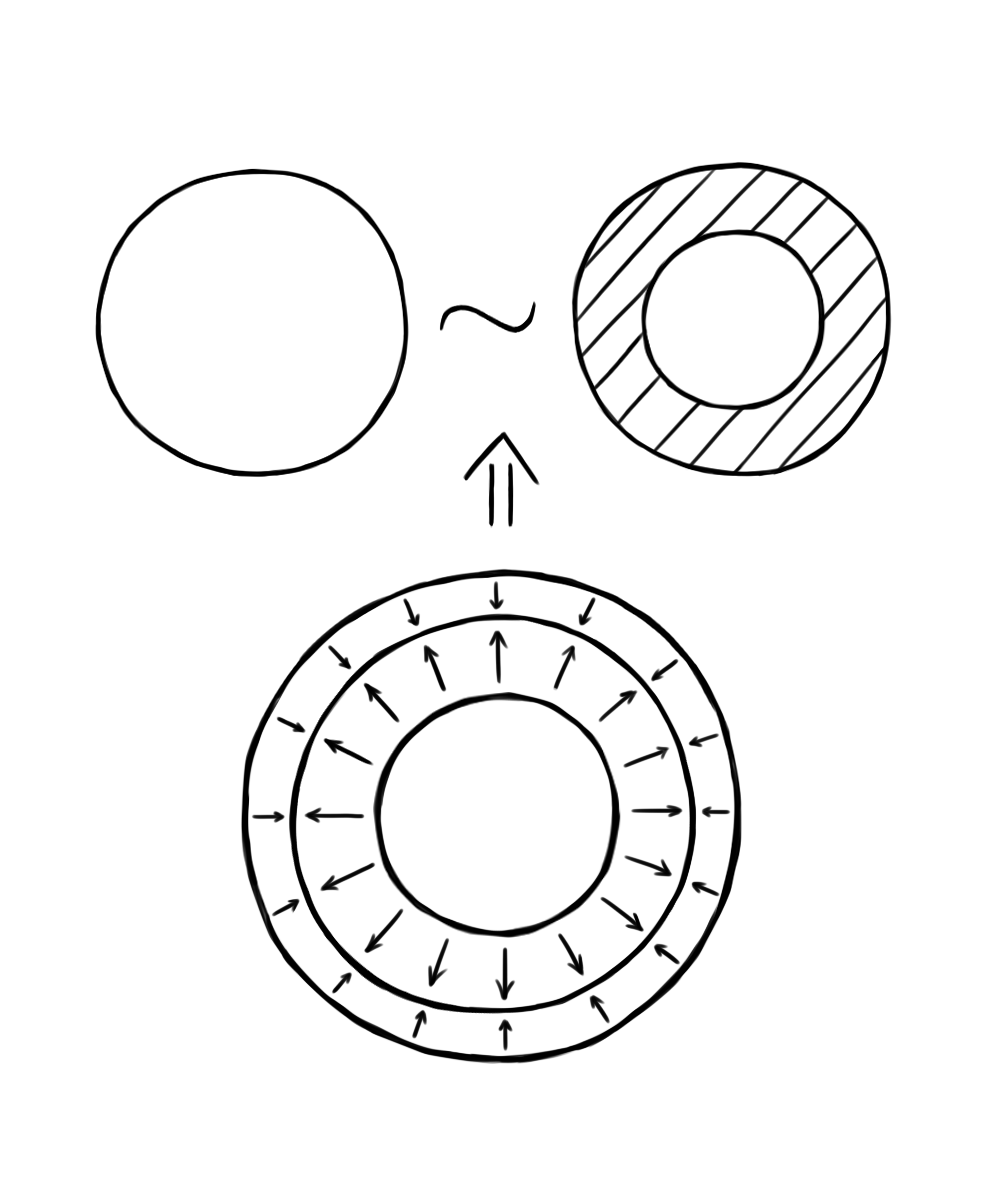
\includegraphics[width=0.5\textwidth]{homotopy-equivalence}
\end{figure}

\begin{definition}
	Пусть $ T $, $ A $ --- топологические пространства и $ A \ssq T $. Тогда $ A $ называется \emph{деформационным
	ретрактом пространства $ T $}, если существует такое непрерывное отображение $ F \colon T \times [0; 1] \to T $,
	что $ f_0 = \Id_T $ и $ f_{1 A} = \Id_A $.
\end{definition}

\begin{remark}
	То есть подпространство $ A $ пространства $ T $ называется деформационным ретрактом, если существует гомотопия
	между $ \Id_T $ и некоторой ретракцией пространства $ T $ на подпространство $ A $.
\end{remark}

\begin{example} Примеры гомотопически эквивалетных пространств:
	\begin{itemize}
		\item любое пространство и любой его деформационный ректракт;
		\item цилиндр и окружность. Кстати, неформально это тоже пространство и деформационный ректракт.
			\begin{figure}[H]
				\centering 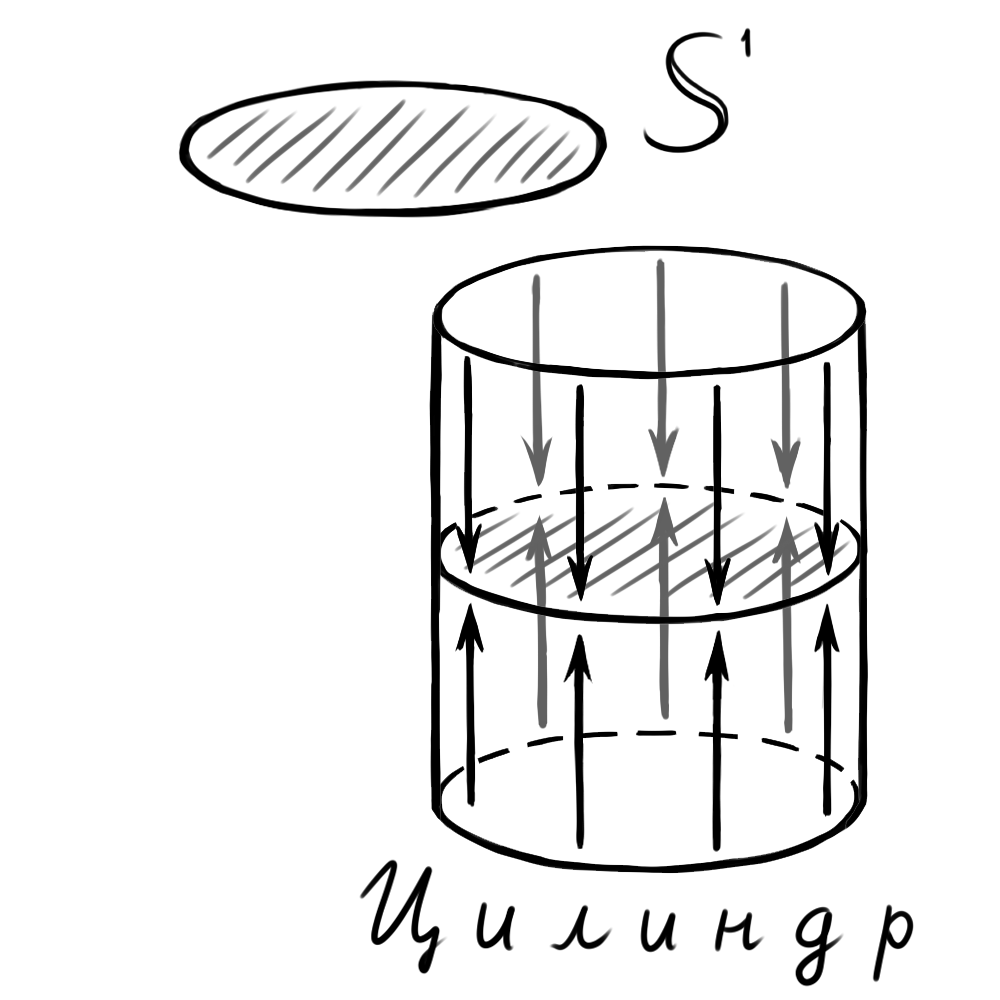
\includegraphics[width=0.5\textwidth]{cylinder-disk}
			\end{figure}
		\item произвольное выпуклое множество $ A \ssq \R^n $ и точка этого множества. Это тоже пространство и
			деформационный ректракт.
			\begin{figure}[H]
				\centering 
\includegraphics[width=0.5\textwidth]{convex-set}
			\end{figure}
	\end{itemize}
\end{example}

\begin{example}
	Применить эту теорию можно следующим образом. В будущем мы докажем, что фундаментальная группа является
	гомотопическим инвариантом. Но известно, что $ \pi_1(\S^1) \simeq \Z $ и $ \pi_1(\pt) \simeq \Set{e} $.
	Значит, $ \S^1 \not \sim \pt $.
\end{example}

\begin{definition}
	Пусть $ T_1 $, $ T_2 $ и $ Z $ --- топологические пространства, а отображение $ f \colon T_1 \to T_2 $ непрерывно.
	Тогда \emph{отображение $ f_* \colon \pi(Z, T_1) \to \pi(Z, T_2) $, индуцированное отображением $ f $},
	определяется следующим образом: для любой петли $ h $ положим $ f_*([h]) = [f \circ h] $.
\end{definition}

\begin{statement}[свойства индуцированных отображений]
	Пусть $ T_1 $, $ T_2 $, $ T_3 $ и $ Z $ --- топологические пространства, а отображения
	$ f, f_1, f_2 \colon T_1 \to T_2 $ и $ f' \colon T_2 \to T_3 $ непрерывны. Тогда:
	\begin{enumerate}
		\item отображение $ f_* $ определено корректно;
		\item если $ f_1 \sim f_2 $, то $ f_{1 *} = f_{2 *} $;
		\item функториальность: $ f'_* \circ f_* = ( f' \circ f )_* $;
		\item если $ f $ осуществляет гомотопическую эквивалентность (то есть для него существует такое
			непрерывное отображение $ g \colon T_2 \to T_1 $, что $ g \circ f = \Id_{T_1} $ и
			$ f \circ g = \Id_{T_2} $), то отображение $ f_* $ взаимно однозначно, причем $ (f_*)^{-1} = g_* $.
	\end{enumerate}
\end{statement}

\begin{proof} \leavevmode
	\begin{enumerate}
		\item Нужно доказать, что если $ h_1 \sim h_2 $, то $ f \circ h_1 \sim f \circ h_2 $. Пусть
			$ H \colon Z \times [0; 1] \to T_1 $ --- гомотопия между $ h_1 $ и $ h_2 $. Тогда отображение =
			$ f \circ H $ является гомотопией между $ f \circ h_1 $ и $ f \circ h_2 $.
		\item Нужно доказать, что для любой петли $ h $ верно $ f_1 \circ h \sim f_2 \circ h $. Пусть
			$ F \colon T_1 \times [0; 1] \to T_2 $ --- гомотопия между $ f_1 $ и $ f_2 $. Определим отображение
			$ h' \colon Z \times [0; 1] \to T_1 \times [0; 1] $: для $ z \in Z $ и $ t \in [0; 1] $ положим
			$ h'(z, t) = (h(z), t) $, то есть $ h' = (h \circ p_1, p_2) $, откуда следует его непрерывность.
			Тогда $ F \circ h' $ есть гомотопия между $ f_1 \circ h $ и $ f_2 \circ h $.
		\item Действительно, для любой петли $ h $ выполнено равенство:
			\[ f'_*(f_*([h])) = f'_*([f \circ h]) = [f' \circ f \circ h] = (f' \circ f)_*([h]). \]
		\item Ясно, что достаточно доказать только <<более того>>. По уже доказанным свойствам имеем:
			\[ g_* \circ f_* = (g \circ f)_* = (\Id_{T_1})_* = \Id_{\pi(Z, T_1)} \text{ ---} \]
			и аналогично в другую сторону. Таким образом, $ (f_*)^{-1} = g_* $.
	\end{enumerate}
\end{proof}

\subsection{Некоторые гомотопические инварианты}

\begin{theorem} \label{the.8.1}
	Пусть $ T_1 $, $ T_2 $ --- топологические пространства, причем пространство $ T_1 $ линейно связно. Тогда
	если $ T_1 \sim T_2 $, то пространство $ T_2 $ тоже линейно связно.
\end{theorem}

\begin{lemma} \label{lem.8.1}
	Множество $ \pi(\pt, T) $ взаимно однозначно соответствует компонентам линейной связности пространства $ T $.
\end{lemma}

\begin{proof}[Доказательство теоремы \ref{the.8.1}]
	По определению гомотопической эквивалентности существуют такие непрерывные отображения $ f \colon T_1 \to T_2 $ и
	$ g \colon T_2 \to T_1 $ таковы, что $ g \circ f \sim \Id_{T_1} $ и $ f \circ g \sim \Id_{T_2} $.
	Из свойств индуцированных отображений при $ Z = \pt $ следует, что $ f_* $ --- биекция между $ \pi(\pt, T_1) $ и
	$ \pi(\pt, T_2) $. Таким образом, эти множества равномощны, а значит, применяя лемму для $ T_1 $ и $ T_2 $,
	находим, что в $ T_2 $ столько же компонент линейной связности, сколько и в $ T_1 $, то есть одна.
\end{proof}

\begin{proof}[Доказательство леммы \ref{lem.8.1}]
	Пусть $ \pt = \Set{t_0} $, где $ t_0 \in T $. Обозначим через $ C(T) $ множество компонент линейной связности
	пространства $ T $, а для каждого $ t \in T $ через $ [t]_C $ все точки, лежащее с $ x $ в одной компоненте
	линейно связности (то есть такие точки, которые можно соединить с $ t $ непрерывным путем).

	Рассмотрим отображение $ \Phi \colon \pi(\pt, T) \to C(T) $, заданное следующим образом: для каждого
	непрерывного отображения $ f \colon \pt \to T $ положим $ \Phi([f]) = [f(t_0)]_C $. Надо проверить,
	что если $ f_1 \sim f_2 $ гомотопны, то $ f_1(t) $ и $ f_2(t) $ в одной компоненте линейной связности.
	Но это очевидно, потому что $ \pt $ состоит из одной точки $ t_0 $, а значит,
	образы соединяются непрерывным путем с помощью гомотопии $ F $ между $ f_1 $ и $ f_2 $.
	Непрерывным путем будет отображение $ f \colon t \mapsto F(t_0, t) $.

	Заметим, что для отображения $ \Phi $ существует обратное $ \Phi^{-1} \colon C(T) \to \pi(\pt, T) $, которое
	можно задать правилом: для $ t \in T $ положим $ \Phi^{-1} = [f_t] $, где $ f_t(t_0) = t $. Таким образом,
	лемма доказана.
\end{proof}

\begin{theorem}
	Пусть $ T_1 $, $ T_2 $ --- топологические пространства. Тогда если $ T_1 \sim T_2 $, то фундаментальные группы
	изоморфны: $ \pi_1(T_1) \simeq \pi_1(T_2) $.
\end{theorem}

\begin{proof} \leavevmode
	\begin{phased}
		\item[Ошибочное доказательство.] По определению гомотопической эквивалентности существуют такие
			непрерывные отображения $ f \colon T_1 \to T_2 $ и $ g \colon T_2 \to T_1 $ таковы,
			что $ g \circ f \sim \Id_{T_1} $ и $ f \circ g \sim \Id_{T_2} $. Тогда при $ Z = [0; 1] $ имеем
			$ f_* \colon \pi_1(T_1) \to \pi_1(T_2) $ и $ g_* \colon \pi_1(T_2) \to \pi_2(T_1) $. Известно,
			что $ (f_* \circ g_*)([\phi]) = (f \circ g)_*([\phi]) = \Id_{\pi_1(T_2)}([\phi]) = [\phi] $, а значит,
			$ g_* = (f_*)^{-1} $.

			Ошибка заключается в том, что $ (f \circ g)_* \neq \Id_{\pi_1(T_2)} $. Дело
			в том, что необходимо смотреть на отображения пар пространств, так как по определению
			$ \pi_1(X, x) = \pi(([0; 1], \Set{0, 1}), (X, \Set{x})) $. В данном случае могла произойти такая ситуация.
			\begin{figure}[H]
				\centering 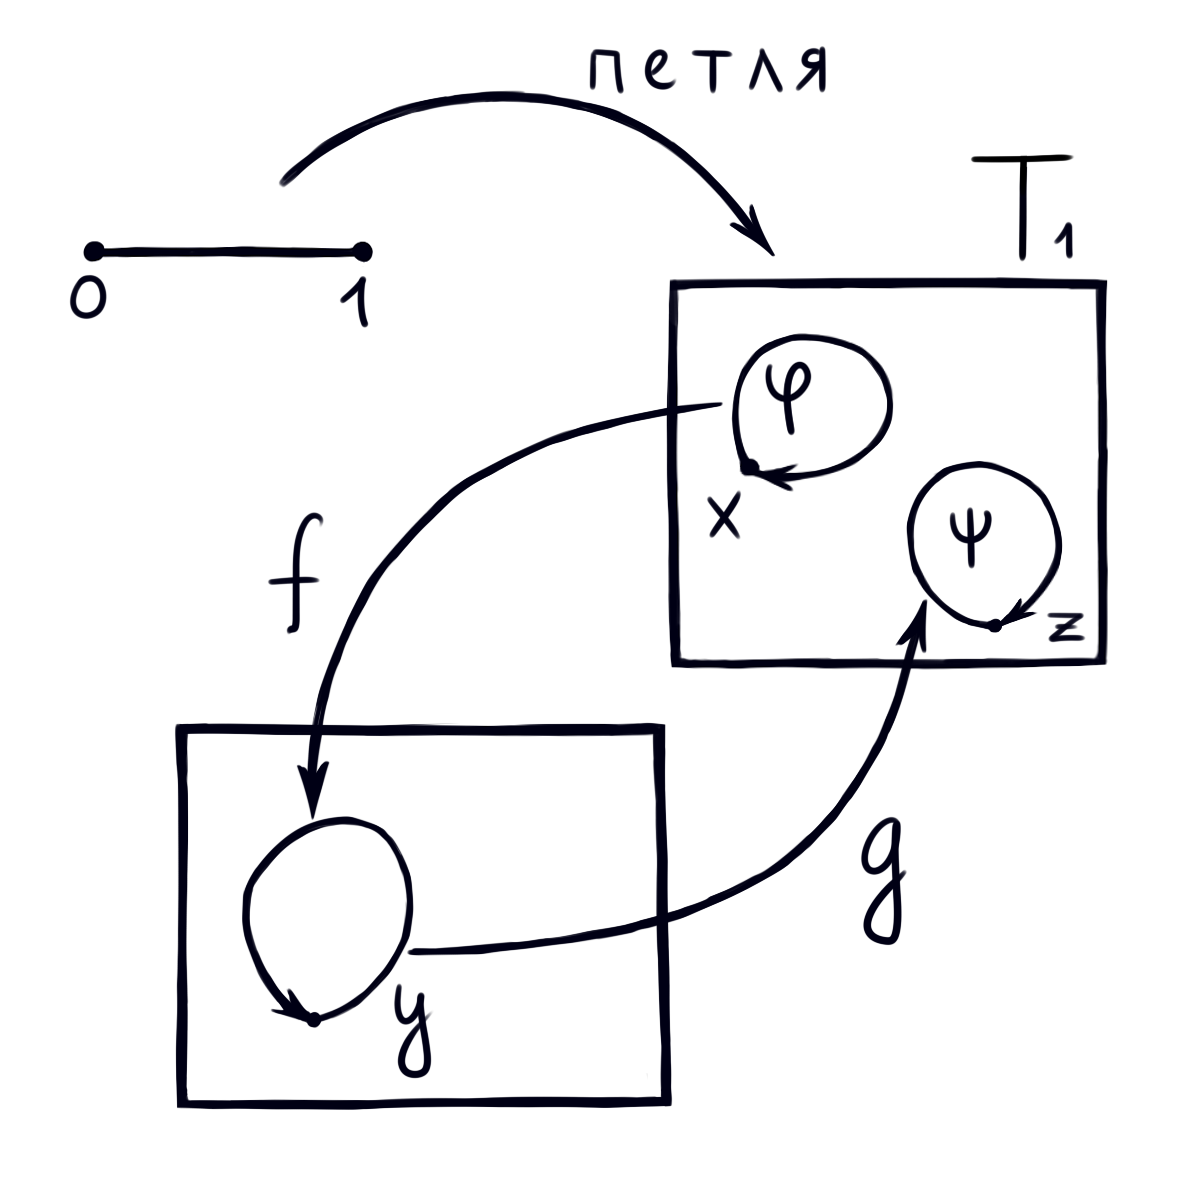
\includegraphics[width=0.5\textwidth]{non-isomorphic}
			\end{figure}
			Петли, конечно, будут гомотопны, но у них может быть разная начальная точка!
		\item[Наброски исправлений.] Итак, пусть $ x, z \in T_1 $, $ y \in T_2 $, тогда
			$ f_* \colon \pi_1(T_1, x) \to \pi_2(T_2, y) $ и $ g_* \colon \pi_1(T_2, y) \to \pi_1(T_1, z) $.
			Пусть $ H \colon T_1 \times [0;1] \to T_2 $ --- гомотопия между $ g \circ f $ и $ \Id_{T_1} $.
			Определим отображение $ \sigma [0; 1] \to T_1 $ следующим образом: для $ t \in [0; 1] $ положим
			$ \sigma(t) = h_t(x) $. Это путь точки $ x $ в процессе гомотопии, так что $ \sigma(0) = x $ и
			$ \sigma(1) = z $. Кроме того, так как гомотопия непрерывна, то и путь $ \sigma $ непрерывен.

			Пусть $ \phi $ --- петля на $ T_1 $ с началом в точке $ x $, а $ \psi \in (g_* \circ f_*)([\phi]) $ ---
			петля на $ T_1 $ с началом в точке $ z $, гомотопная петле $ \phi $. Определим петлю $ \chi $,
			которая сначала проходит путь от $ x $ до петли $ \chi $, затем саму петлю и, наконец,
			возвращается обратно в точку $ x $:
				\[ \chi(t) = \begin{cases}
						\sigma(4 t),
							& \text{если } t \in \left[ 0; \frac{1}{4} \right]; \\
						\psi\left(2 t - \frac{1}{2}\right),
							& \text{если } t \in \left[ \frac{1}{4}; \frac{3}{4} \right]; \\
						\sigma(4-4 t),
							& \text{если } t \in \left[ \frac{3}{4}; 1 \right].
					\end{cases}
				\]
			\begin{remark}
				Здесь можно было брать любые границы, лишь бы все части отрезка не вырождались в точку.
			\end{remark}
			\begin{figure}[H]
				\centering 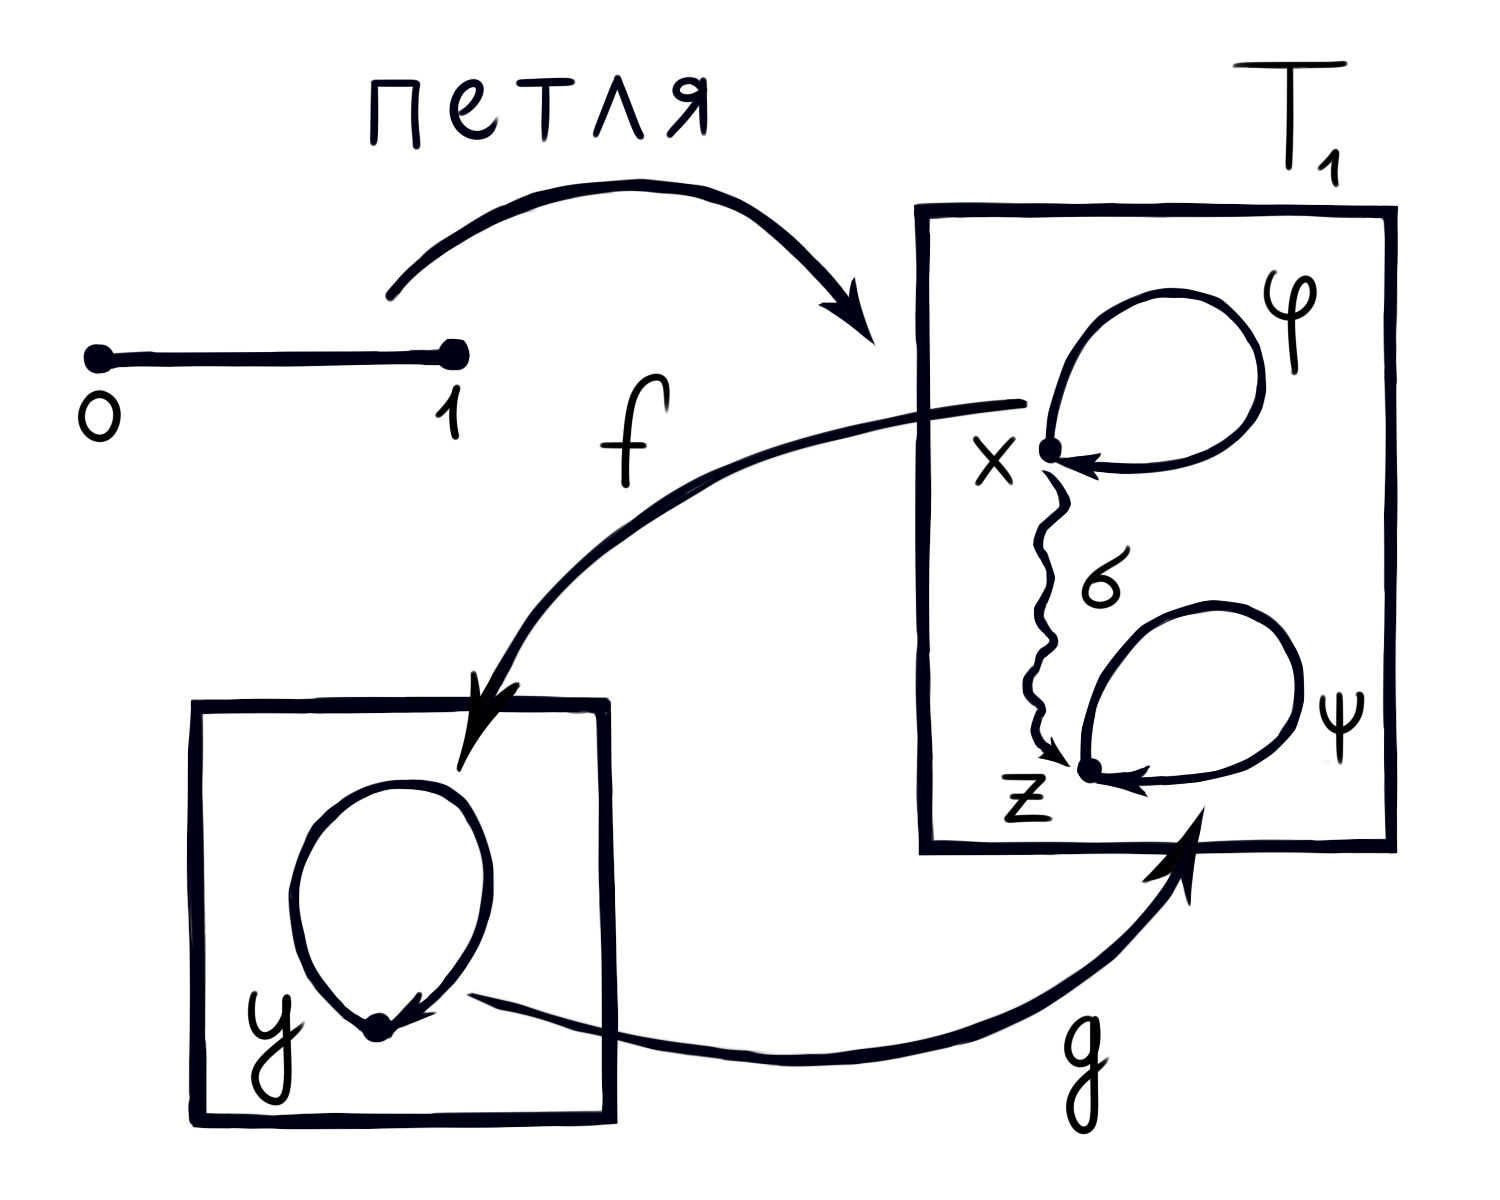
\includegraphics[width=0.5\textwidth]{non-isomorphic-fixed}
			\end{figure}
			Наконец, построим отображение $ h $: для каждой петли $ \phi $ положим
			$ h([\phi]) = [\chi] $. Остается только:
			\begin{enumerate}
				\item доказать, что это отображение корректно, то есть если $ \phi_1 \sim \phi_2 $,
					то $ \chi_1 \sim \chi_2 $ при любом выборе $ \chi_1 $ и $ \chi_2 $ (это, в общем-то, тривиально,
					так как мы брали $ \chi_1 \sim \phi_1 $ и $ \chi_2 \sim \phi_2 $);
				\item проверить, что отображение $ h $ удовлетворяет соотношению
					$ h \circ g_* \circ f_* = \Id_{\pi_1(T_1, x)} $;
				\item доказать, что отображение $ h \circ g_* \circ f_* $ является изоморфизмом групп.
			\end{enumerate}
			Для доказательства последнего пункта можно  построить обратное отображение. Например, аналогично, с
			помощью такого отображения $ h' $, что $ h' \circ f_* \circ g_* = \Id_{\pi_1(T_2, y)} $.
	\end{phased}
\end{proof}

\end{document}
